\documentclass[hide notes,intlimits]{beamer}

\mode<presentation>
{
  \usetheme[footline]{UAFshadealert}
  \setbeamercovered{transparent}
}

% frames are 128 millimeters by 96 millimeters

% load packages
\usepackage[english]{babel}
\usepackage[latin1]{inputenc}
\usepackage[T1]{fontenc}
\usepackage{amsmath,amssymb,wasysym}
\usepackage{lmodern}

\usepackage{tikz}
\usetikzlibrary{shapes,arrows,shadows}

\usepackage{empheq}
\usepackage{color}
\usepackage{animate}

\graphicspath{{figures/}}

% Some useful commands (from MPL)
\newcommand{\s}[1]{\ensuremath{\,\text{#1}}}
\newcommand{\unit}[1]{\ensuremath{\,\text{#1}}}

\definecolor{dark red}{HTML}{E41A1C}
\definecolor{dark green}{HTML}{4DAF4A}
\definecolor{dark violet}{HTML}{984EA3}
\definecolor{dark blue}{HTML}{084594}
\definecolor{dark orange}{HTML}{FF7F00}
\definecolor{light blue}{HTML}{377EB8}
\definecolor{light red}{HTML}{FB9A99}
\definecolor{light violet}{HTML}{CAB2D6}

\setbeamercolor{boxed}{fg=black,bg=uaf yellow}


\newenvironment{transbox}{%
  
\begin{tikzpicture}
    \node[drop shadow,rounded corners,text width=\textwidth,fill=white, fill opacity=0.6,text opacity=1] \bgroup
  }{
    \egroup;\end{tikzpicture}} 

\newenvironment{transbox-tight}{%
  \begin{tikzpicture}
    \node[drop shadow,rounded corners,fill=uaf yellow, fill opacity=0.75,text opacity=1] \bgroup
  }{
    \egroup;\end{tikzpicture}} 


% title page
\title[]{Better subglacial hydrology into PISM}
\subtitle{(the Parallel Ice Sheet Model)}

\author[Bueler \and van Pelt]{Ed Bueler\inst{*} and Ward van Pelt\inst{\dagger}}
\institute{\inst{*} University of Alaska Fairbanks \and %
           \inst{\dagger} IMAU, Utrecht, Netherlands}
%\author[Bueler]{Ed Bueler}
%\institute{University of Alaska Fairbanks}

\date{IGS June 2012}


\begin{document}

% define what is shown at the beginning of each section
%\AtBeginSection[]
%{
% \begin{frame}<beamer>
%   \frametitle{Outline}
%   \tableofcontents[currentsection,subsectionstyle=hide/hide/hide]
% \end{frame}
%}


\setbeamertemplate{background canvas}
{
  \tikz{\node[inner sep=0pt,opacity=1.0] {\includegraphics[width=\paperwidth]{uaf_beamer_shade_bg}};}
} 

% insert titlepage
\begin{frame}
  \titlepage
\end{frame}

\setbeamertemplate{background canvas}
{
  % empty
}

%\begin{frame}
%   \frametitle{Outline}
%   \tableofcontents[subsectionstyle=hide/hide/hide]
%\end{frame}


\newcommand{\scream}[1]{\alert{\textbf{#1}}}

\begin{frame}
  \frametitle{PISM = Parallel Ice Sheet Model}

  \begin{center}
      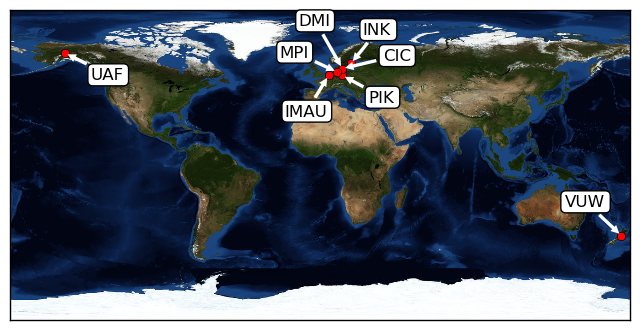
\includegraphics[width=80mm]{figs/pism-users-map}
  \end{center}

\vspace{-2mm}
  \begin{itemize}
  \item \alert{\large\texttt{www.pism-docs.org}}  and  \url{help@pism-docs.org}
  \item runs on laptops to supercomputers
  \item documented releases once a year
  \item \emph{User's Manual} with real modeling examples including Greenland Ice Sheet, Ross Ice Shelf, and St\"orglaciaren
  
  \bigskip
  \scriptsize
  \item[$\circ$] supported by the NASA Modeling, Analysis and Prediction (grant NNX09AJ38G)
  \item[$\circ$] jointly developed by UAF and the Potsdam Institute for Climate Impact Research
  \end{itemize}
\end{frame}


\newcommand{\whytitle}{why we need better subglacial hydrology}

\begin{frame}
  \frametitle{\whytitle}
  \framesubtitle{motivation 1}

\begin{center}
  we are \scream{NOT} conserving mass (of liquid water)
\end{center}

\begin{columns}
\begin{column}{0.5\textwidth}
  \begin{itemize}
    \item current basal water scheme is a ``can'' of porous till $\longrightarrow$
      \begin{itemize}
        \item[$\circ$] ``overflows'' at 2m of water \dots overflow lost
        \item[$\circ$] but models till strength in reasonable way (Tulaczyk et al 2000)
      \end{itemize}
    \item no lateral transport of water
    \item model is most suitable for (e.g.) Siple coast ice streams $\longrightarrow$
  \end{itemize}
\end{column}
\begin{column}{0.5\textwidth}
FIXME: can of till

\vspace{15mm}

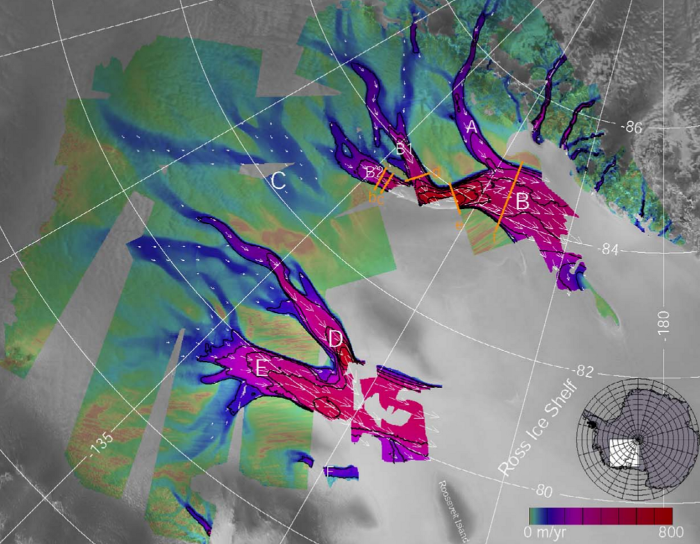
\includegraphics[width=0.7\textwidth]{figs/siple}
\end{column}
\end{columns}
\end{frame}


\begin{frame}
  \frametitle{\whytitle}
  \framesubtitle{motivation 2}
  
\begin{center}
  we \scream{ARE} conserving energy (better than before)
\end{center}
  
  \begin{itemize}
    \item better energy conservation using enthalpy
    \item generates new basal melt rate equation
    \item \emph{lots of water comes from dissipating gravitational potential energy, and some from geothermal energy}
  \end{itemize}

  \begin{center}
    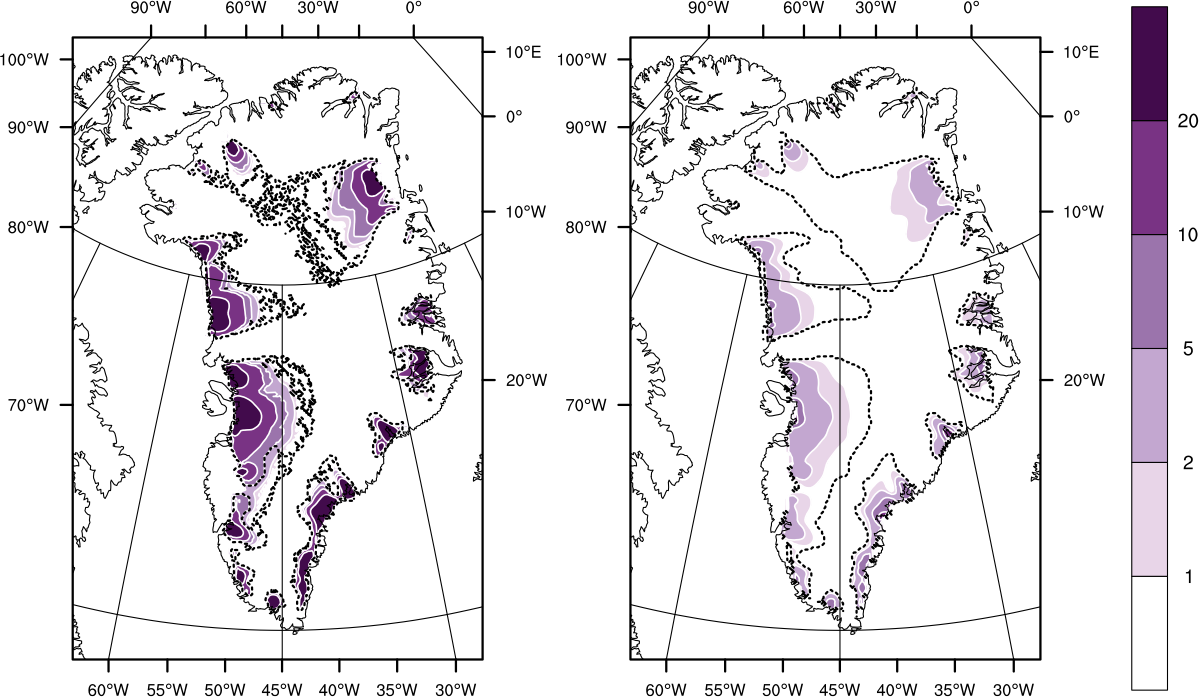
\includegraphics[height=0.4\textheight]{figs/enthalpy-model-crop}
    
    \medskip
    \scriptsize \textbf{left}: basal melt rate using \underline{enthalpy} \qquad \textbf{right}: basal melt rate using \underline{temperature}

    \tiny (from Aschwanden et al (2012) \emph{An enthalpy formulation for glaciers and ice sheets}, J. Glaciol.)
  \end{center}
\end{frame}


\newcommand{\goaltitle}{what we want to do for users}


\begin{frame}
  \frametitle{\goaltitle}
  \framesubtitle{goal 1}
  
\begin{center}
  \scream{give users reasonable default behavior}
\end{center}
  
  \begin{itemize}
    \item that does no harm
  \end{itemize}
\end{frame}


\begin{frame}
  \frametitle{\goaltitle}
  \framesubtitle{goal 2}
 
\begin{center}
  \scream{report the amount of subglacial water delivered at each outlet}
\end{center}
  
  \begin{itemize}
    \item we can do this for ice flow because we know which direction the ice flows
    \item we need a subglacial hydrology just to know which fjord gets the water
  \end{itemize}

\begin{center}
\bigskip

    FIXME: side-by-side drainage basins for $h$ and for $\psi$
\end{center}

\end{frame}


\begin{frame}
  \frametitle{\goaltitle}
  \framesubtitle{goal 3}

\begin{center}
   \scream{provide a playground for testing basal sliding models}
\end{center}
  
  \begin{itemize}
    \item FIXME:  show results from van Pelt \& Oerlemans
  \end{itemize}
\end{frame}



\begin{frame}
  \frametitle{these goals clash}

\begin{itemize}
\item you can't please all the people all the time
\end{itemize}
\end{frame}


\begin{frame}
  \frametitle{elements of subglacial hydrology}
  \framesubtitle{we can agree on these?}

\newcommand{\bq}{\mathbf{q}}

  \begin{itemize}
    \item \textbf{conservation of mass}:
    
    $$W_t + \nabla \cdot \bq = m / \rho_w$$

where $W=$ thickness of water sheet, $\bq=$ flux, $m=$ supply rate

    \item \textbf{hydraulic potential} for top of water sheet:
    
    $$\phi = p_w + \rho_w g (b + W)$$

where $\phi=$ hydraulic potential, $b=$ bedrock elevation

    \item \textbf{Darcy flow}:
    
    $$\bq = - \frac{K W}{\rho_w g} \nabla \phi$$
    
    \scriptsize or \quad $\bq = - k W^\alpha |\nabla \phi|^{\beta - 2} \nabla \phi$ \quad etc.
    
\normalsize where $K$ hydraulic conductivity (\emph{not} constant in general)
  \end{itemize}

\end{frame}


\begin{frame}
  \frametitle{elements of subglacial hydrology}
  \framesubtitle{whence pressure?}

  \begin{itemize}
    \item an equation determines the pressure; some alternatives:
      \begin{itemize}
      \item[$\circ$]
        $$P = \rho_i g H$$
      \item[$\circ$]
        $$P = \rho_i g H \left(\frac{W}{W_{\text{crit}}}\right)^\gamma$$
      \item[$\circ$]  physical models for opening (wall melt, sliding) and closure (creep)
        
        FIXME: Hewitt generic equation

  elliptic equation determines water pressure

      \item[$\circ$] bounds on pressure
        
        FIXME: Schoof et al inequalities

  elliptic variational inequality determines water pressure
      \end{itemize}
  \end{itemize}

\end{frame}


\begin{frame}
  \frametitle{time scales with the simple choice}

  \begin{itemize}
    \item FIXME: combined equation for $W$: comment
    \item hydraulic potential from three elevations:
    \begin{align*}
      \phi &= \rho_i g H + \rho_w g (b+W) \\
           &= \rho_i g \underline{\phantom{|}h\phantom{|}} + (\rho_w - \rho_i) g \underline{\phantom{|}b\phantom{|}} + \rho_w g \underline{\phantom{|}W\phantom{|}}
    \end{align*}
    \item FIXME: equation for $\mathbf{v}$: comment \& show results
  \end{itemize}

\end{frame}


\begin{frame}
  \frametitle{results from the simple choice}

  \begin{itemize}
    \item FIXME: show for EAIS
  \end{itemize}

\end{frame}











\begin{frame}
  \frametitle{FIXME: ideas to include}

\scriptsize
  \begin{itemize}
  \item channeling flow can only be implemented in a 2d framework when the position of the channels is predefined; this does not seem to be desirable in our approach
  \item main problem at the moment is the interaction/feedback of the water flux and the wall melt term in the opening/closure-equation. This interaction ultimately leads to concentrated water flow in infinitely narrow channels (larger water flux ->  larger channel -> lower pressure -> larger water flux)
  \item We leave out the wall melt term in the closure relation and hence only model linked-cavity flow (opening by cavitation balanced by creep closure). This model would be suitable for all regions of an ice sheet except for fast flowing outlet glaciers.
  \item Make the wall melt opening term in the opening/closure-relation a function of the water input rate rather than the water flux.
  \item \alert{great danger} in building a model whose parameters cannot be identified
  \end{itemize}
\end{frame}








\end{document}
